\documentclass[a4paper]{article}

%% Language and font encodings
\usepackage[english]{babel}
\usepackage[utf8]{inputenc}
\usepackage{ragged2e}

% for figures
\usepackage{graphicx}
\usepackage[font=small]{caption}

% for hyperlinks
\usepackage[colorlinks = true,
            linkcolor = blue,
            urlcolor  = blue,
            citecolor = blue,
            anchorcolor = blue]{hyperref}

% for pseudocode
\usepackage{algorithm}
\usepackage{algpseudocode}
% for coloring
\usepackage[usenames,dvipsnames,svgnames]{xcolor}

% bibliography
\usepackage[backend=biber,citestyle=authoryear,maxcitenames=1,maxbibnames=10,natbib]{biblatex}
\addbibresource{FDTD_paper.bib}

% paragraph spacing
\setlength{\parindent}{0em}
\setlength{\parskip}{1em}

\begin{document}

\title{Simulating electromagnetic wave propagation in ice with finite difference time domain}
\author{Ben Hills}
\maketitle

\justify
\textbf{Abstract:} Radio-echo sounding is a common field application for recovering information about the subsurface by transmitting an electromagnetic wave and measuring the returning signal. 
Here, we develop a simple numerical model using finite difference time domain to simulate electromagnetic wave propagation. We test this model in several scenarios to observe behavior of the propagating wave. The model is built from a general framework, but applications of this method are developed for use
in ice penetrating radar studies. Radio-echo sounding techniques are commonly used on ice sheets to recover information about ice thickness, internal stratigraphy, and vertical strain rates to mention a few. Some of the applications of finite difference time domain and more generally of radio-echo sounding in ice are discussed. 

\raggedright
\section{Introduction}

Light and the electromagnetic wave have been of particular interest to physicists throughout the modern age of science. In the $17^{th}$ century, Isaac Newton shattered our conception of light and color with a prism and a rainbow. A couple hundred years later, Micheal Faraday and James Clerk Maxwell made great contributions to the experimental and theoretical understanding of electromagnetism, respectively. Eventually, their discoveries put Newton's visible light in its appropriate position on
the electromagnetic spectrum. While his original intentions were theoretical, Maxwell's equations inspired a technological revolution which inevitably shaped the world in which we live.

Today we lean heavily on a thorough understanding of electromagnetism. Our vast communication networks, including the internet and cellular phone technology, are in the simplest sense a series of electromagnetic signals relayed from one position to another. Other practical applications include the X-ray, the microwave, radar, etc. Moreover, an appreciation of the electromagnetic spectrum has expanded on our scientific knowledge, a greater understanding of the Earth's energy balance is one example.

Geoscientists utilize the concepts of electromagnetism as well. A common field methodology called radio-echo sounding (RES) uses radar waves to recover information about subsurface features. The basic concept of RES is that an electromagnetic pulse is transmitted at the Earth surface, or from the air, and its returning signal is measured through time. The time and power of the returning wave are used to decipher information about the material through which it is travelling.
Unfortunately, interpreting RES data is not always simple. The three dimensionality of the wave as well as heterogeneities in the substrate through which the wave moves can complicate the returning signal.

Here, we summarize a numerical method to simulate Maxwell's equations called finite difference time domain. When leveraged appropriately, these types of numerical simulations can develop our intuition about physical phenomena. In this particular, case we want to better understand the intricacies of electromagnetic wave propagation in a heterogeneous and nonuniform domain. Starting from the basic equations, we formulate a numerical model in both one and two dimensions. In
this study, the model is only used for simple scenarios, but with further development it can be used for more complicated situations. We analyze our results and place them in the context of research applications through a discussion on ice penetrating radar. 

\section{Methods}

\subsection{Maxwell's Equations}

We use Maxwell's equations to simulate the propagation of an electromagnetic wave. We take a particular interest in propagation through ice, but the overall model formulation is the same for any material. Following \citet{Griffiths1981}, Maxwell's equations are written as, 

\begin{equation}
    \nabla \times \textbf{E} = - \frac{\partial \textbf{B}}{\partial t}
    \label{eqn:E}
\end{equation}
\begin{equation}
    \nabla \times \textbf{H} = \textbf{J} + \frac{\partial \textbf{D}}{\partial t}
    \label{eqn:H}
\end{equation}

Here, \textbf{E} and \textbf{H} are the electric and magnetic fields, respectively, and t is time. All other vectors are related to \textbf{E} and \textbf{H} through the constitutive equations, 

\begin{equation}
    \textbf{B} = \mu \textbf{H} 
    \label{eqn:CM}
\end{equation}
\begin{equation}
    \textbf{D} = \epsilon \textbf{E} 
    \label{eqn:CE}
\end{equation}
\begin{equation}
    \textbf{J} = \sigma \textbf{E}   
    \label{eqn:Ohm}
\end{equation}

Equation~\ref{eqn:CM} relates the magnetic field to magnetic inductance, \textbf{B}, through the magnetic permeability, $\mu$. Equation~\ref{eqn:CE} relates the electric field to electric inductance, \textbf{D}, through the electric permittivity, $\epsilon$. The electric permittivity and the magnetic permeability together tell us something about the velocity of light through the media of interest, $c=\sqrt{1\slash {\mu \epsilon}}$. Lastly, equation~\ref{eqn:Ohm}, sometimes called Ohm's Law,
relates the electric field to the current, \textbf{J}, through the electric conductivity, $\sigma$. 

Each of the vectors in these equations has three components, meaning that the material constants (i.e. $\mu$ and $\epsilon$) are really nine-component tensors. Therefore, the two field equations (~\ref{eqn:E} and~\ref{eqn:H}) break down into six separate partial differential equations,

\begin{equation}
    \frac{\partial E_z}{\partial y} - \frac{\partial E_y}{\partial z} = -\left( \mu_{xx}\frac{\partial H_x}{\partial t} + \mu_{xy}\frac{\partial H_y}{\partial t} + \mu_{xz}\frac{\partial H_z}{\partial t} \right)
\end{equation}

\begin{equation}
    \frac{\partial E_x}{\partial z} - \frac{\partial E_z}{\partial x} = -\left( \mu_{yx}\frac{\partial H_x}{\partial t} + \mu_{yy}\frac{\partial H_y}{\partial t} + \mu_{yz}\frac{\partial H_z}{\partial t} \right)
\end{equation}

\begin{equation}
    \frac{\partial E_y}{\partial x} - \frac{\partial E_x}{\partial y} = -\left( \mu_{zx}\frac{\partial H_x}{\partial t} + \mu_{zy}\frac{\partial H_y}{\partial t} + \mu_{zz}\frac{\partial H_z}{\partial t} \right)
\end{equation}

\begin{equation}
    \frac{\partial H_z}{\partial y} - \frac{\partial H_y}{\partial z} = \left( \sigma_{xx} E_x +\sigma_{xy} E_y +\sigma_{xz} E_z \right) + \left( \epsilon_{xx}\frac{\partial E_x}{\partial t} + \epsilon_{xy}\frac{\partial E_y}{\partial t} + \epsilon_{xz}\frac{\partial E_z}{\partial t} \right)
\end{equation}

\begin{equation}
    \frac{\partial H_x}{\partial z} - \frac{\partial H_z}{\partial x} = \left( \sigma_{yx} E_x +\sigma_{yy} E_y +\sigma_{yz} E_z \right) + \left( \epsilon_{yx}\frac{\partial E_x}{\partial t} + \epsilon_{yy}\frac{\partial E_y}{\partial t} + \epsilon_{yz}\frac{\partial E_z}{\partial t} \right)
\end{equation}

\begin{equation}
    \frac{\partial H_y}{\partial x} - \frac{\partial H_x}{\partial y} = \left( \sigma_{zx} E_x +\sigma_{zy} E_y +\sigma_{zz} E_z \right) + \left( \epsilon_{zx}\frac{\partial E_x}{\partial t} + \epsilon_{zy}\frac{\partial E_y}{\partial t} + \epsilon_{zz}\frac{\partial E_z}{\partial t} \right)
\end{equation}

Of course, in most situations the above equations are simplified based on symmetry within the problem. 

\begin{figure}
    \centering
    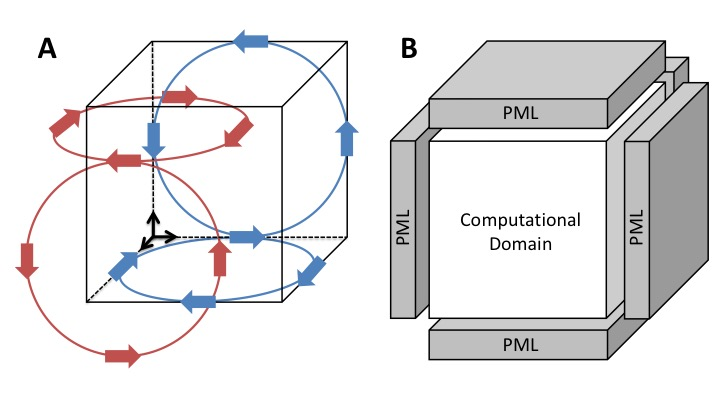
\includegraphics[width=\textwidth]{./Figures/Methods_Figure.jpg}
    \caption{Cartoon representations of the numerical method. a) The Yee Grid discretization technique. The electric field (red) is staggered by half a spatial step from the magnetic field (blue). b) The perfectly matched layer boundary condition is a region where the material constants are changed in order to artificially attenuate the electromagnetic wave.}
    \label{fig:YeePML}
\end{figure}

\subsection{Finite Difference Time Domain}

Except in the most simple cases, the six partial differential equations above have no analytic solution. Instead, problems are solved numerically. Here we use a finite difference method (Appendix) commonly referred to as finite difference time domain. Finite differencing is fairly common practice in numerical methods, but solving Maxwell's Equations in this way is unique because there are two interdependent fields to be updated in time. Care is taken to construct the numerics in order to force the electromagnetic field to propagate as a wave, a physically realistic representation. Next we will discuss some of the details of this method. 

\subsubsection{Yee Grid}

First, we must discretize a grid on which the numerical problem will be solved. We start in three dimensions, but eventually simplify the problem into a lower dimensionality. The most common discretization technique is using what is called a Yee Grid \citep{Yee1966}. This grid has two separate discretizations for the electric and magnetic fields (Figure~\ref{fig:YeePML}a). Those two fields are staggered in space, allowing a more accurate calculation of the curl at each node. As an
example, take vector $E_x$. The time rate of change of $E_x$ is dependent on the curl of $\textbf{H}$. In Figure~\ref{fig:YeePML}a we see that $E_x$, and all $\textbf{E}$-vectors for that matter, is centered in curling loops of the $\textbf{H}$-field. Thus, we can use $\textbf{H}$-vectors to calculate the curl, as in $\frac{\partial H_z}{\partial y} - \frac{\partial H_y}{\partial z}$. The same is true for updating $\textbf{H}$ from $\textbf{E}$.

The Yee grid is also staggered in time. Only a half time step, $\frac{\Delta t}{2}$, is taken between the calculation of the magnetic field from the electric field, and the same for the electric field from the magnetic field. Therefore, a full time step is taken between each new update of either field from its own previous state. This progressive stepping allows the electromagnetic wave to propagate in a physical manner. When deciding the time step, some attention must be given to numerical stability. The Courant-Friedrichs-Lewy stability criterion (CFL) says that 

\begin{equation}
    \sqrt{(\Delta x)^2 + (\Delta y)^2 + (\Delta z)^2} > \sqrt{\frac{1}{\mu \epsilon}} \Delta t
\end{equation}

where $\Delta x$, $\Delta y$, and $\Delta z$, are the spatial steps in each direction. This stability criterion requires that the time step is limited by the spatial grid. 

\begin{figure}
    \centering
    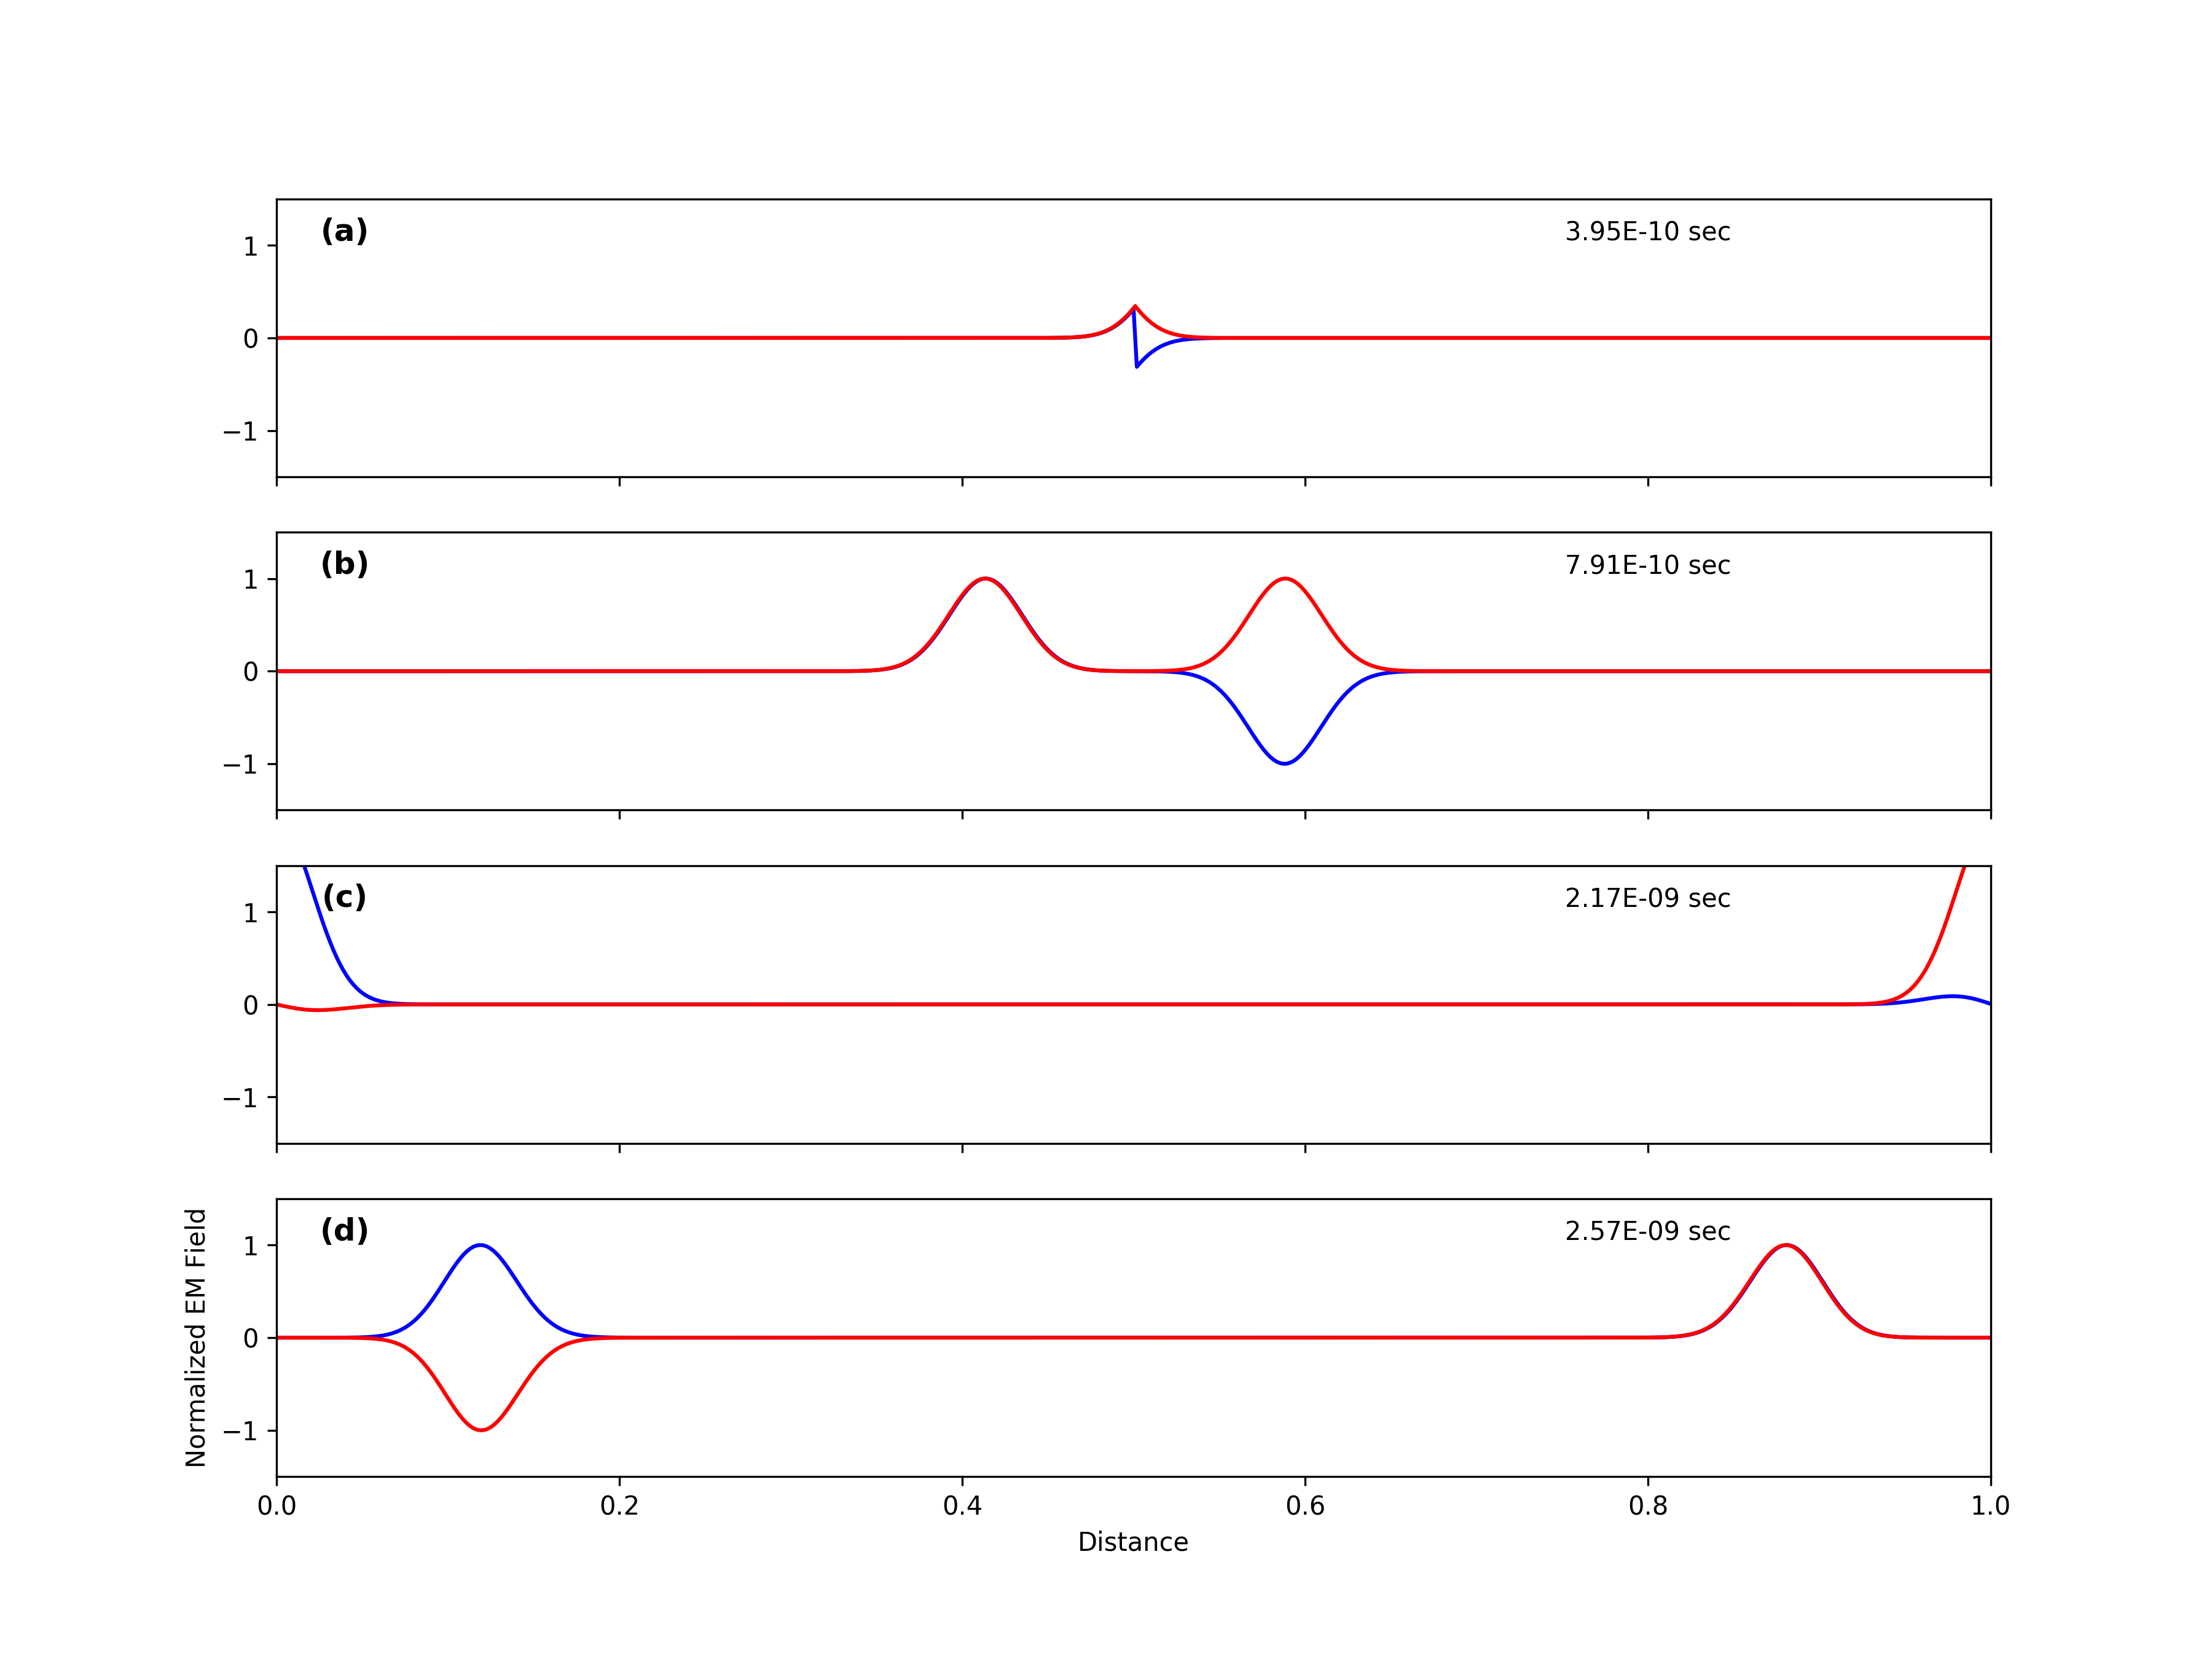
\includegraphics[width=\textwidth]{./Figures/DirichletBC.png}
    \caption{A sequence of plots for the one-dimensional finite difference time domain simulation with Dirichlet boundary conditions. In each panel the normalized electric field (red) and the magnetic field (blue) are shown.}
    \label{fig:Dirichlet}
\end{figure}

\subsubsection{FDTD Modes}

Now that we have the full three-dimensional problem description and we have the Yee Grid discretization technique, we will simplify the field equations in order to apply them to specific problems. To start, we will make two assumptions which apply to all subsequent descriptions. First, we assume that the off-diagonal components of the permeability and permittivity tensors are zero. This assumption means that each curl calculation only forces change in its right handed direction. Second, we assume that there is no current in the material (i.e. $\textbf{J}=0$). 

Carrying those two assumptions, we will next build finite difference update equations that can be implemented numerically for both a one-dimensional and a two-dimensional case. In the one-dimensional case we use z as our only direction in the grid. The field equations then simplify so that only the partial derivatives $\frac{\partial}{\partial z}$ and $\frac{\partial}{\partial t}$ are nonzero. The set of six equations then reduces to four, and those four can be further divided into two groups
based on the vectors that remain in each equation. We will write out only one group here, the $E_y-H_x$ mode, but know that there is an analogous $E_x-H_y$ mode. The choice of one over another is unimportant in our case. For the $E_y-H_x$ mode, the six equations reduce to two,

\begin{equation}
    \frac{\partial E_y}{\partial z} = \mu_{xx} \frac{\partial H_x}{\partial t}
\end{equation}

\begin{equation}
    \frac{\partial H_x}{\partial z} = \epsilon_{yy} \frac{\partial E_y}{\partial t}
\end{equation}

These equation can then be transformed into update equations by substituting the finite difference representation for each derivative, 

\begin{equation}
    \frac{\left. E_y \right\vert_t^{k+1} - \left. E_y \right\vert_t^{k}}{\Delta z} = \mu_{xx}^{k} \frac{\left. H_x \right\vert_{t+\frac{\Delta t}{2}}^{k} - \left. H_x \right\vert_{t-\frac{\Delta t}{2}}^{k}}{\Delta t}
\end{equation}

\begin{equation}
    \frac{\left. H_x \right\vert_{t+\frac{\Delta t}{2}}^{k} - \left. H_x \right\vert_{t+\frac{\Delta t}{2}}^{k-1}}{\Delta z} = \epsilon_{yy}^{k} \frac{\left. E_y \right\vert_{t+\Delta t}^{k} - \left. E_y \right\vert_{t}^{k}}{\Delta t}
\end{equation}

and rearranging for the update of $E_y$ and $H_x$ vectors in time, 

\begin{equation}
    \left. H_x \right\vert_{t+\frac{\Delta t}{2}}^{k} = \left. H_x \right\vert_{t-\frac{\Delta t}{2}}^{k} + \frac{\Delta t}{\mu_{xx}^{k}} \frac{\left. E_y \right\vert_{t}^{k} - \left. E_y \right\vert_{t}^{k-1}}{\Delta z} 
\end{equation}

\begin{equation}
    \left. E_y \right\vert_{t+\Delta t}^{k} = \left. E_y \right\vert_{t}^{k} + \frac{\Delta t}{\epsilon_{yy}^{k}} \frac{\left. H_x \right\vert_{t+\frac{\Delta t}{2}}^{k} - \left. H_x \right\vert_{t+\frac{\Delta t}{2}}^{k-1}}{\Delta z} 
\end{equation}

For two dimensions there is an analogous procedure. Here, we express the $E_z$ mode which describes a grid in only the x and y directions. The magnetic field vectors will be solved in those same directions, but the electric field vectors will be solved in the z-direction, 

\begin{equation}
    \frac{\partial E_z}{\partial y} = - \mu_{xx} \frac{\partial H_x}{\partial t}
\end{equation}

\begin{equation}
    \frac{\partial E_z}{\partial x} = \mu_{yy} \frac{\partial H_y}{\partial t}
\end{equation}

\begin{equation}
    \frac{\partial H_y}{\partial x} - \frac{\partial H_x}{\partial y} = \epsilon_{zz} \frac{\partial E_z}{\partial t}
\end{equation}

and again the equations used for updating the vectors in time will be,

\begin{equation}
    \left. H_x \right\vert_{t+\frac{\Delta t}{2}}^{i,j} = \left. H_x \right\vert_{t-\frac{\Delta t}{2}}^{i,j} + \frac{\Delta t}{\mu_{xx}^{i,j}} \frac{\left. E_z \right\vert_{t}^{i+1,j} - \left. E_z \right\vert_{t}^{i,j}}{\Delta x} 
\end{equation}

\begin{equation}
    \left. H_y \right\vert_{t+\frac{\Delta t}{2}}^{i,j} = \left. H_y \right\vert_{t-\frac{\Delta t}{2}}^{i,j} + \frac{\Delta t}{\mu_{yy}^{i,j}} \frac{\left. E_z \right\vert_{t}^{i,j+1} - \left. E_z \right\vert_{t}^{i,j}}{\Delta y}
\end{equation}

\begin{equation}
    \left. E_z \right\vert_{t+1}^{i,j} = \left. E_z \right\vert_{t}^{i,j} + \frac{\Delta t}{\epsilon_{zz}^{i,j}} \left(
\frac{\left. H_y \right\vert_{t+\frac{\Delta t}{2}}^{i,j} - \left. H_y \right\vert_{t+\frac{\Delta t}{2}}^{i-1,j}}{\Delta x} - \frac{\left. H_x \right\vert_{t+\frac{\Delta t}{2}}^{i,j} - \left. H_x \right\vert_{t+\frac{\Delta t}{2}}^{i,j-1}}{\Delta y} \right)
\end{equation}

\begin{figure}
    \centering
    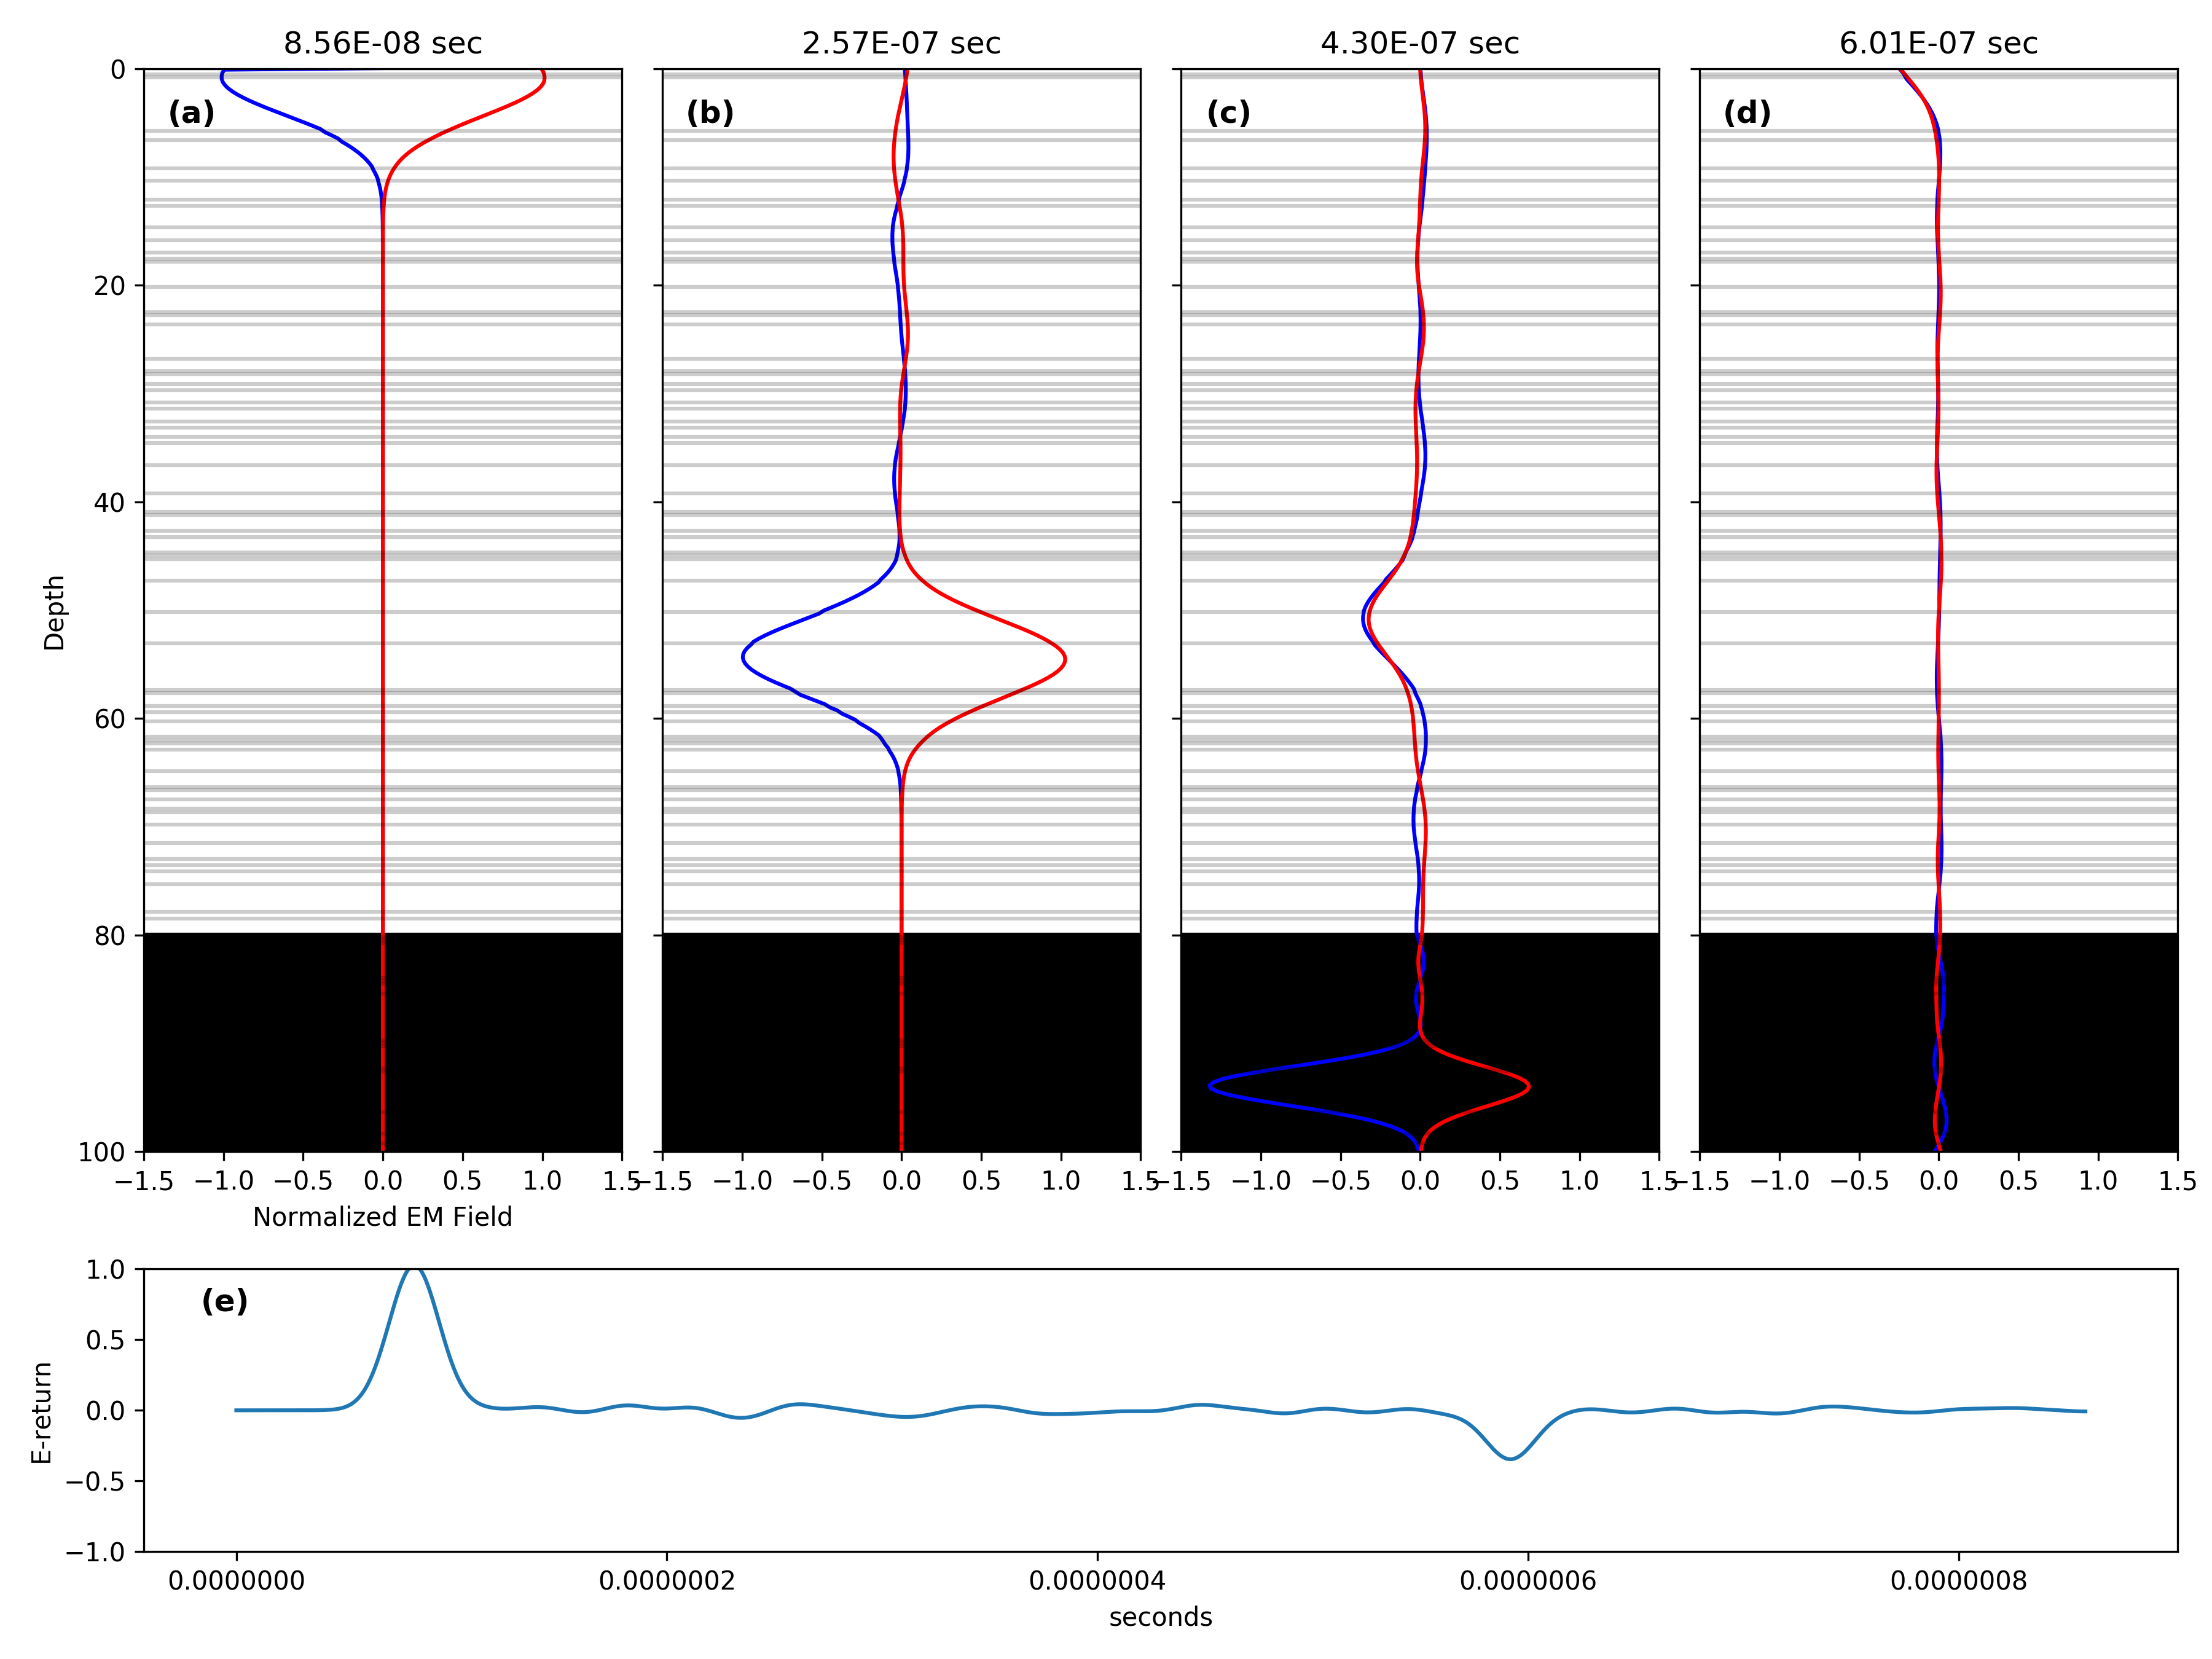
\includegraphics[width=\textwidth]{./Figures/IceSimulation.png}
    \caption{Simulation of EM wave propagation through ice. a-d) A time series of the electric field (red) and magnetic field (blue) as the wave propagates through the ice column. Layers of debris (lower permittivity) are shown by horizontal gray lines and the bed is shown as the dark gray region below 80 m. e) The return of the electric field measured at the surface through time.}
    \label{fig:Ice}
\end{figure}

\subsubsection{Boundary Conditions}

The final step for the full numerical description is to apply the boundary conditions. The most simple boundary condition is a fixed boundary, or Dirichlet condition. In that case, all nodes along the boundary will remain fixed at their initial state for all time. This type of boundary condition causes wave reflection because the fixed node forces a gradient along the edge. Alternatively, in some scenarios we do not want the wave to reflect. Another option is to use a boundary condition called a perfectly matched layer. Here, we follow the wave as it is approaching the boundary and match its gradient so that it can move off the page. Take some pseudocode for a one-dimensional model, 

\begin{center}
    \colorbox[RGB]{239,240,241}{
    \begin{minipage}{.8\linewidth}
        \begin{algorithmic}[H]
            \State H1, H2, H3 = 0, 0, 0
            \State E1, E2, E3 = 0, 0, 0
            \State
            \For{t in TimeArray}
            \State Hx[-1] += (dt/(dz*mu[-1]))*(E3 - Ey[-1]) 
            \State Ey[0] += (dt/(dz*epsilon[-1]))*(Hx[0] - H3) 
            \State
            \State H3, H2, H1 = H2, H1, Hx[0]
            \State E3, E2, E1 = E2, E1, Ey[-1]
            \EndFor
        \end{algorithmic}
    \end{minipage}}
\end{center}

Here, we define values for the electric and magnetic field at the boundaries. Those values are saved for the current state as well as for the previous two states (i.e. H1, H2, H3). The curl at the boundary is then calculated using that saved state from two time steps previous, thus artificially forcing the gradient which will move the wave out of the domain. 

As seen here, the perfectly matched layer boundary condition is relatively easy to implement in one dimension. However, it becomes much more complex at higher dimensions. At higher dimensionality the wave may be approaching the boundary at an angle, so it is not enough to simply save the previous state and use that to `fake' a gradient. In higher dimensions we introduce something called a stretching variable, which is set to unity in the main computational domain but progressively damped toward
the edges. The stretching variable creates an artificial attenuation of the wave as it gets closer to the actual boundary.  

\section{Results}

Three model scenarios were run using the finite difference time domain formulation described here. Two of these simulations are one-dimensional, and the third is a preliminary simulation with the two-dimensional model. First, we carry out the most simple case in one dimension with Dirichlet boundary conditions and constants for free space (Figure \ref{fig:Dirichlet}). The electromagnetic wave is initiated with a Gaussian source added to the electric field in the center of the model domain.
Through time the wave moves toward the boundary at the speed of light ($\sqrt{\frac{1}{\mu \epsilon}}$). When the wave hits the boundary it is reflected. Depending on which boundary, the sine of the wave could be flipped upon reflection. In our case we see that the electric wave gets flipped on the left hand wall and the magnetic on the right hand wall. 

The second simulation uses constants for ice (Figure \ref{fig:Ice}). Here, we simulate electromagnetic wave propagation in a scenario that would be typical of ice penetrating radar. This simulation is also changed from the first in that we now use a perfectly matched layer boundary condition so that the wave moves out of the domain. This ice domain has variable constants that represent debris layers in the ice column and then bedrock at 80 m. Those contrasts in permittivity cause the
electromagnetic wave to reflect as it slows down or speeds up. Each reflection moves back toward the surface. In Figure\ref{fig:Ice}e we plot the return of the electric field through time. The outgoing pulse is emitted around $8e^{-08}$ seconds, and we can see that the returning wave from the bed arrives at about $6e^{-07}$ seconds. Taking the time difference and assuming a roughly constant wave speed through the ice will give us the distance to the bed. In this case, the actual speed may be a little bit off of the realistic value because the debris layer permittivity was amplified to show more contrast. 

Finally, we develop a two-dimensional algorithm. This simulation is kept simple because the perfectly matched layer boundary was too complex in two dimensions to do for this project. However, for the simple case of Dirichlet boundary conditions we see a similar result to the one-dimensional case (Figure \ref{fig:2D}). Again, we transmit a Gaussian source in the lower left quadrant of the domain. Through time, the wave moves toward the boundaries and is eventually reflected. As in one
dimension, the sign of the wave is flipped when it hits a wall. 

\begin{figure}
    \centering
    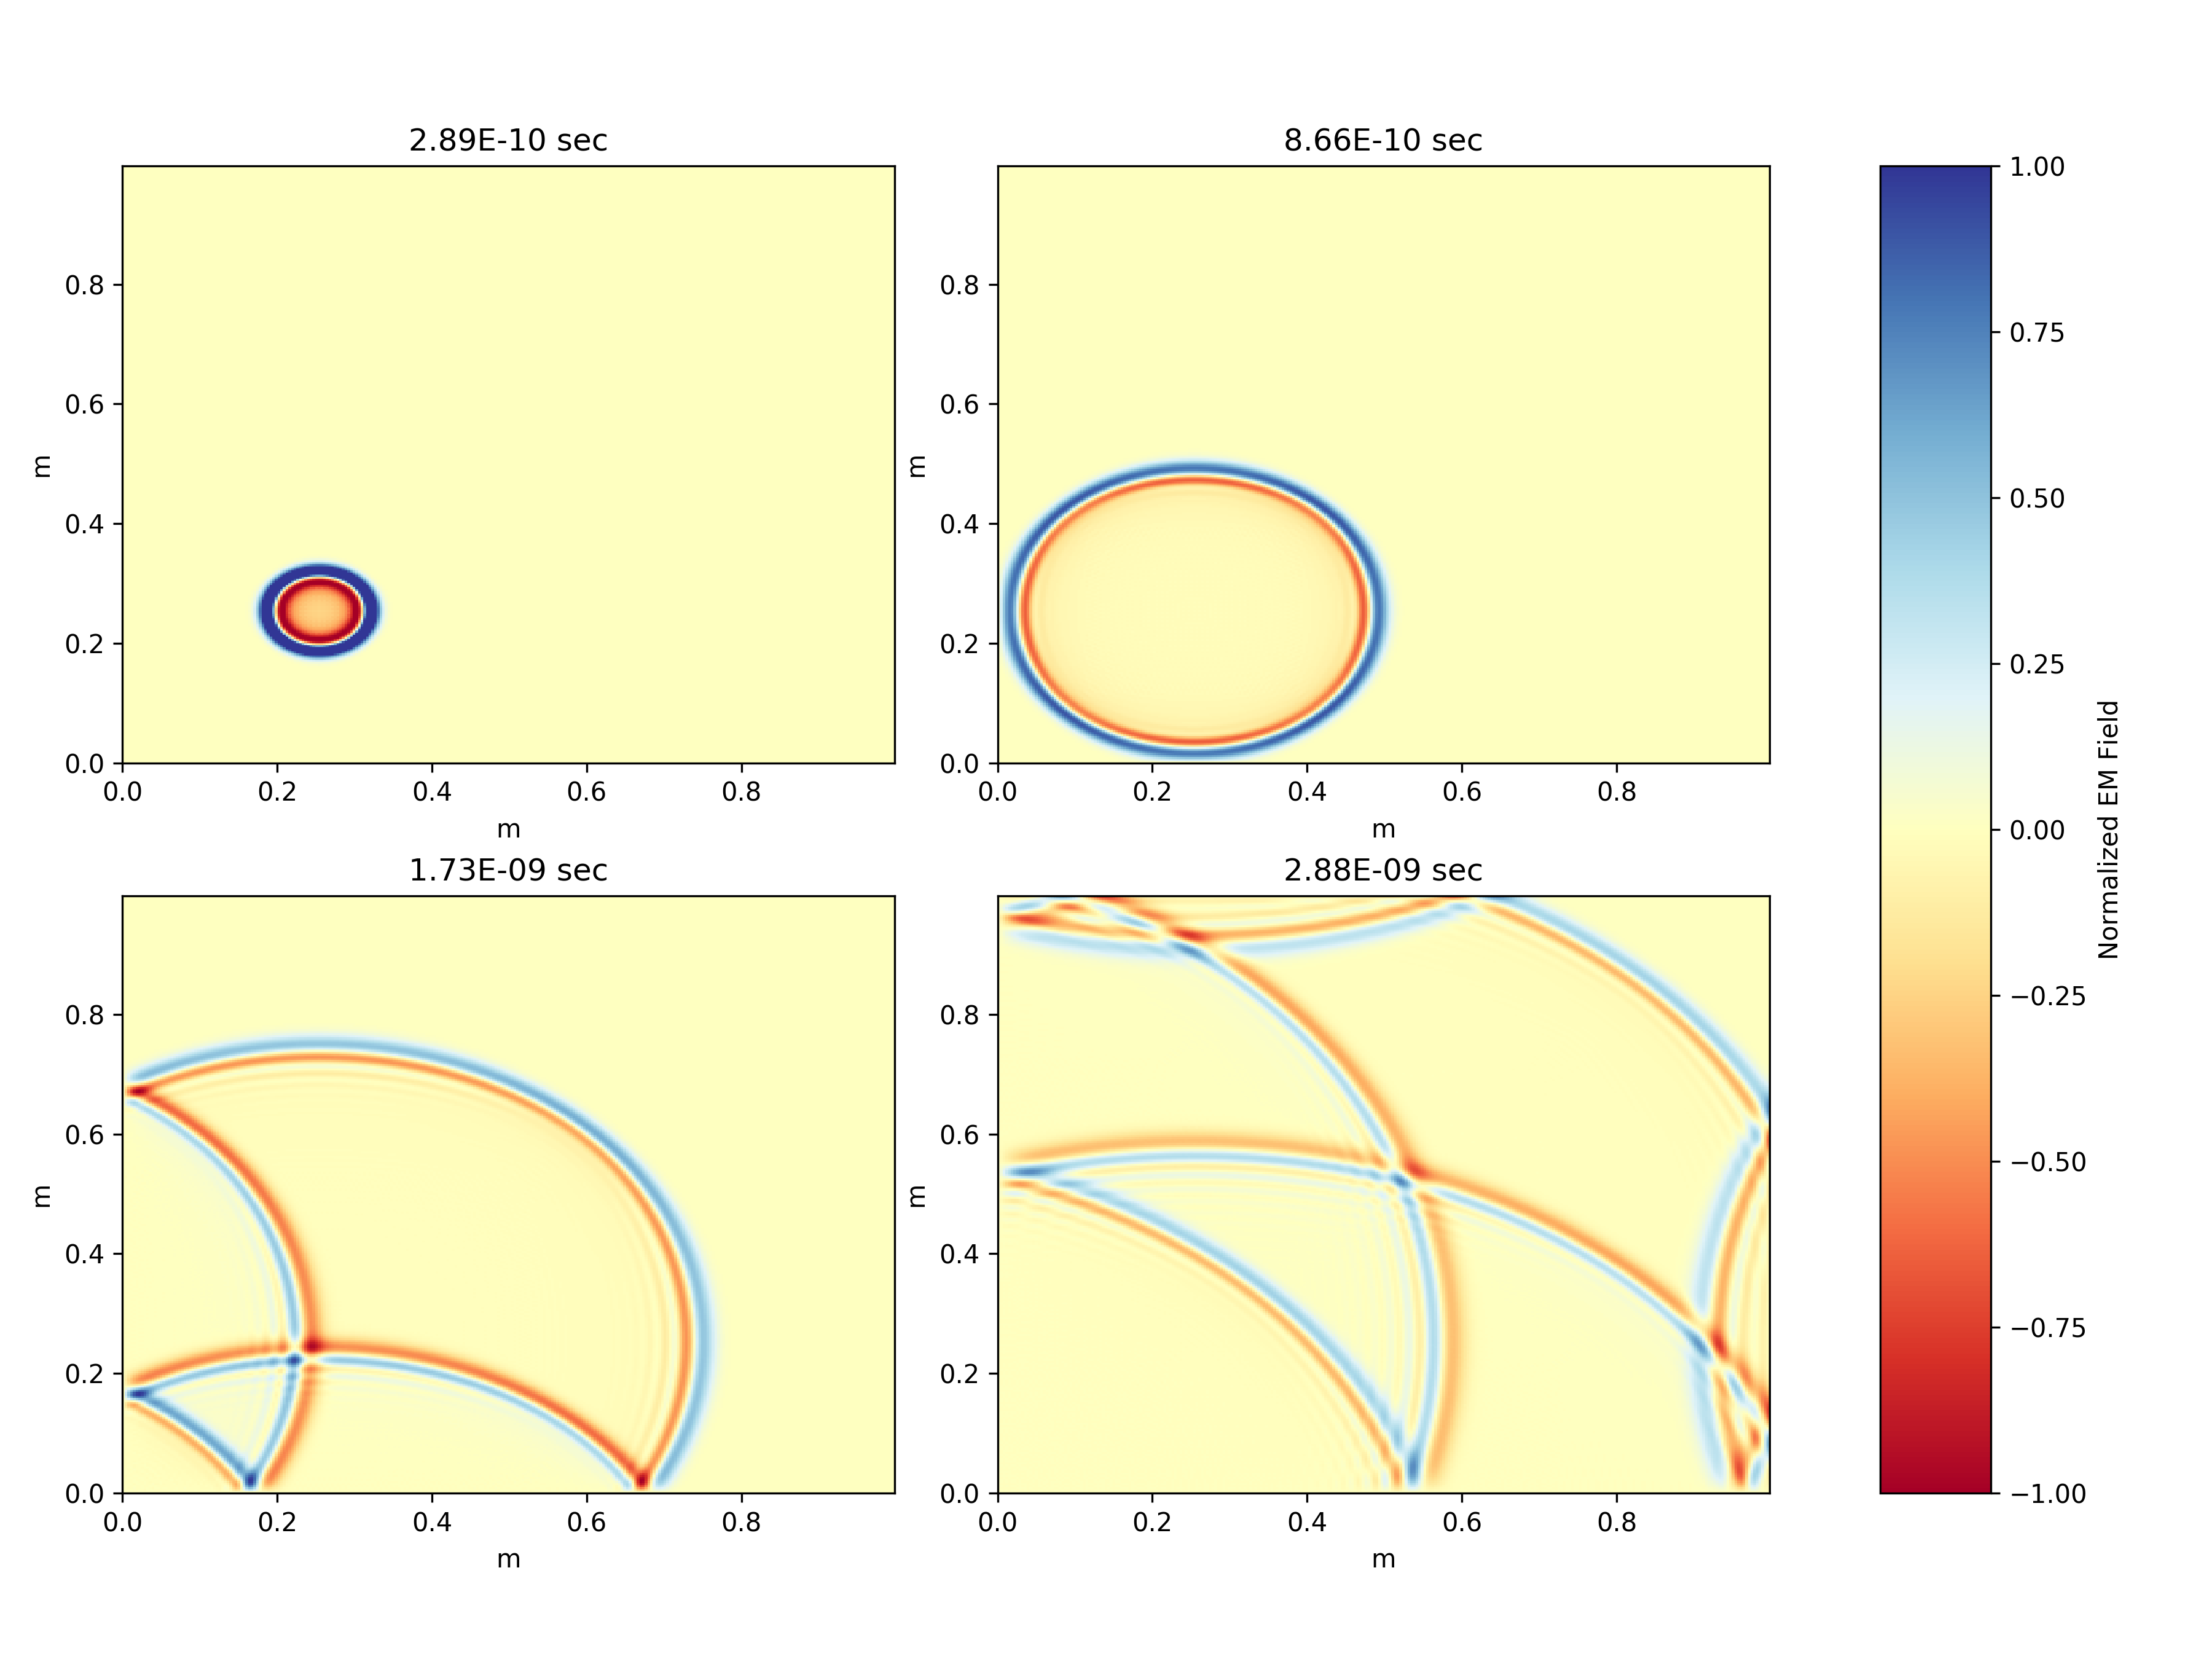
\includegraphics[width=\textwidth]{./Figures/2D_figure.png}
    \caption{A two-dimensional simulation of electromagnetic wave propagation with Dirichlet boundary conditions. Together, the panels show a time progression of the wave propagation through the domain.}
    \label{fig:2D}
\end{figure}

\section{Discussion}

While the potential applications of this modeling study are general to any media, we will discuss the more specific applications in glaciology. RES methods are commonly used to infer information from the interior of an ice sheet. Importantly, this type of data collection is logistically easier than the alternative of drilling boreholes through the ice sheet. Being relatively simple and inexpensive, RES can be done for a large area. These methods have been utilized in glaciology since it was discovered that radio waves propagate long distances through ice \cite{Evans1961}, and similar seismic methods were even used before then \cite{Robin1958}. 

The most basic glaciological information that is recovered from RES includes mapping ice thickness and depicting internal layers. One particularly interesting example of internal layers giving strong information was the first observation of what has been come to be known as the `Raymond bump' \citep{Vaughan1999}. Those authors could infer variation in vertical strain rates around the ice divide. Based on Raymond's original theory, vertical strain rates are lowest right at the divide because of the low deviatoric stress of ice in that region. 

Looking forward, we know that there is a lot of development to be made in the ways that RES data are used. The amount of information captured by the electromagnetic wave is greatly underutilized; only the lowest hanging fruit are generally taken. One example of innovation in RES techniques is using phase-based RES to more accurately measure vertical strain rates \citep{Nicholls2015,Kingslake2014}. Here, two antennas are placed at the ice surface, both of which measure the returning wave. The two antennas are joined by one computer which carefully measures the difference in phase. This new piece of information adds accuracy to the knowledge of the subsurface, and is being used to more precisely measure vertical strain rates.

A second innovation in RES utility is in measuring wave attenuation with distance travelled through the ice. The strength of the signal is attenuated due to free charge carriers, polar molecule orientation, and lattice vibration within the ice \citep{Dowdeswell2004}. The rate of that attenuation is dependent on intrinsic properties of the ice such as temperature and impurity content \citep{MacGregor2007}. An Arrhenious relation relates the attenuation rate to each of those intrinsic properties. Consider
temperature,

\begin{equation}
N_a \propto exp(E_0/kT)
\end{equation}

where $N_a$ is the attenuation rate, $E_0$ is the activation energy, $k$ is Boltzmann’s constant, $T$ and is temperature. Based on this equation, spatial variations in the attenuation rate can hypothetically be used to infer spatial variations in ice temperature \citep{MacGregor2012}. In fact, this method has been used to map depth-averaged temperatures throughout a large portion of the Greenland ice sheet \citep{Macgregor2015}.

Seeing these two innovative areas of development in the methodology, it is apparent that RES data can be confusing. In order to interpret the recovered information in a way that the data are usable, we must properly understand the physics of electromagnetic wave propagation. This is where modeling techniques such as finite difference time domain provide an opportunity to test our intuition. The model can be used to create artificial data for simple scenarios \citep{Irving2006}. One specific example in ice uses finite difference time domain to test bed characteristics and determine the returning signal at the surface \citep{Christianson2016}

\section{Conclusions}

In this preliminary study, we simulate propagation of an electromagnetic wave using finite difference time domain. Several simple scenarios were carried out in one and two dimensions. As expected, we see a strong control of model behavior based on the boundary conditions that are implemented. For Dirichlet boundary conditions, the wave is reflected off of the boundary. On the other hand, the perfectly matched layer boundary condition allows the wave to propagate out of the domain. Because of its utility for testing intuition on radar wave propagation, there is potential for this numerical method to be used in ice-penetrating radar studies to test scenarios in which the recovered data do not meet our initial intuition. 

\pagebreak
\section{Appendix: Finite Difference Method}

One common method to solve partial differential equations numerically is with finite differences. This appendix is meant to give a brief overview of how this method works. Finite differencing uses the Taylor Series which approximates a function $f$ at a point $x_i$, 

\begin{equation}
    f(x_i + \Delta x_i) = f(x_i) + \Delta x_i \left. \frac{\partial f}{\partial x} \right\vert_{x_i} + \frac{\Delta x_i^2}{2!} \left. \frac{\partial^2 f}{\partial x^2} \right\vert_{x_i} + \dots
\end{equation}

From the Taylor Series above, we can solve for any order derivative by simply moving terms around. 

\begin{equation}
    \left. \frac{\partial f}{\partial x} \right\vert_{x_i} = \frac{f(x_i + \Delta x_i) - f(x_i)}{\Delta x_i} + O(\Delta x_i)
\end{equation}

where $O(\Delta x_i)$ is the error associated with removing higher order terms. With this equation we can substitute points on the grid (right-hand side) for a partial derivative (left-hand side) in some partial differential equation. This allows us to numerically solve complex problems. 

\pagebreak
\section*{Data Availability}

Model scripts are available for download as a git repository at \url{https://github.com/benhills/FDTD.git}.

\printbibliography

\end{document}
